\documentclass[11pt]{article}

\usepackage[margin=1in]{geometry}
\usepackage{amsmath, amssymb, amsthm}
\usepackage{booktabs}
\usepackage{graphicx}
\usepackage{hyperref}
\usepackage{mathtools}

% Shared theorem environments and notation for the WP1-WP4 papers.
% Requires amsthm (and amsmath/amssymb) to be loaded before \input.

\newtheorem{theorem}{Theorem}
\newtheorem{lemma}{Lemma}
\newtheorem{remark}{Remark}


\title{Dissecting Objective Mismatch in Model-Based RL:\\
  \large Bias-Variance Decomposition and Value-Gradient Diagnostic}
\author{Firmansyah Sundana, Novanto Yudistira}
\date{WP1 revision}

\begin{document}
\maketitle

\begin{center}
\textbf{Status:} WP1 revision, superseding the tabular-only Draft~v2. All numbers are
produced by the committed runs under \texttt{runs/} (each with a \texttt{manifest.json}
pinning the config, git SHA, and library versions). The work is aligned to the WP1--WP4
plan (value-aware loss stabilization and scalability for MBRL); WP1 --- the
weight-estimator theory, mismatch diagnostics, and VJP profiling --- is complete and
summarised in \texttt{paper/wp1/notes/wp1\_report.md}. The continuous neural transfer
(Exp~4) is superseded by the MuJoCo Exp~1.1 of Sec.~\ref{sec:exp11-deep}; its earlier
numbers remain withdrawn.
\end{center}

\begin{abstract}
Model-based reinforcement learning fits a dynamics model to predict the next state,
typically by maximum likelihood, and then uses that model to improve a policy. The
objective mismatch problem~\cite{lambert2020objective} is that the model's likelihood
need not correlate with its ability to guide the policy. Value-aware model learning
(VaGraM~\cite{voelcker2022vagram}) reweights the model loss by the value function, but
is empirically known to sometimes underperform MLE. We isolate \emph{when and why} this
happens. We contribute (i) a corrected theory of the weighted ratio estimator $w$: the
first-order variance penalty for value-aware weighting is
$\sigma_w^2\,\mathrm{Var}(V)/n$ (not $\sigma_w^2\,\mathbb{E}[V^2]/n$ as previously
stated), and this dominance result holds only for the uncapacitated fixed estimator ---
under a finite-capacity model, reweighting reallocates capacity and can \emph{reduce}
Bellman risk; (ii) a controlled synthetic benchmark, Distractor-Gym, with a functional
distractor family (linear/nonlinear/stochastic) and a configurable model-capacity knob
(a reduced-rank feature-budget transition model); and (iii) two quantitative
diagnostics --- policy-gradient alignment (cosine between true and model-induced
gradients) and the
$\lvert\delta_{\mathrm{TD}}\rvert \sim \lVert \nabla V\rVert \cdot \varepsilon_{\mathrm{model}}$
decomposition. We find that (a)~with an uncapacitated model the decomposition holds
($R^2 = 0.98$ dense, $0.76$--$0.81$ sparse) and is invariant to the distractor count
because deterministic distractors are fit exactly and $\nabla_{s_d} V = 0$;
(b)~with a capacity-limited model and unpredictable (stochastic) distractors, MLE
policy-gradient alignment collapses as the distractor count grows (e.g.\ $\cos$ from
$0.86$ at $d_d=0$ to $-0.08$ at $d_d=2$), while value-aware weighting --- especially
VAML-1/Lambert --- restores it (to $0.16$--$0.34$), whereas gradient-only VaGraM does
not; and (c)~the prediction-risk dominance of MLE is confined to the uncapacitated
estimator (estimated-weight Bellman risk $\ge$ MLE in $100\%$ of uncapacitated regimes)
and fails for capacity-limited fitting ($50\%$/$33\%$ for VaGraM/VAML-1). For depth we
add (iv)~WP1 diagnostics on a differentiable MuJoCo Distractor-Gym --- an exact
policy-gradient alignment measurement (Exp~1.1) and a per-sample VJP profiling harness
(Exp~1.2). The deep alignment degrades with the distractor count, and exact online VJP is
dispatch-bound on commodity hardware, where stale-weight caching recovers the overhead.
\end{abstract}

\section{Introduction}

Model-based RL (MBRL) is a sample-efficient framework for continuous
control~\cite{deisenroth2011pilco,janner2019mbpo,hafner2023dreamerv3,hansen2024tdmpc2}.
A dynamics model is fit to predict one-step transitions and then used by a policy or
planner. The standard objective for the model is maximum likelihood (MLE), which
minimizes prediction error uniformly over the state space. Lambert
et~al.~\cite{lambert2020objective} showed this objective can be \emph{mismatched} with
the downstream goal: the one-step likelihood is not always correlated with control
performance.

A principled family of remedies --- value-aware model learning
(VAML~\cite{farahmand2017vaml,farahmand2018itervaml}; VaGraM~\cite{voelcker2022vagram})
--- reweights the model loss by the value function, so that the model is accurate
\emph{where value changes}. VaGraM showed these losses help under small model capacity
and distracting state dimensions, yet the literature also documents regimes in which
value-aware losses \emph{underperform} MLE~\cite{voelcker2022vagram,cvaml2025,romi2026}.
There is currently no isolated, controlled characterization of when and why value-aware
weighting fails, and no modern diagnostic suite ported to current baselines.

This revision makes the following contributions:

\begin{enumerate}
\item \textbf{Corrected theory of the weight estimator.} The value-aware weight
  $w = w(V, \nabla V)$ is estimated from finite data and is a random variable with bias
  and variance. We prove (i) a \emph{prediction-risk} result for the weighted ratio
  estimator: the correct first-order variance penalty is
  $\sigma_w^2\,\mathrm{Var}(V)/n$, and MLE dominance holds for the uncapacitated fixed
  estimator but \emph{not} for finite-capacity model fitting (Theorem~\ref{thm:pred});
  (ii) an \emph{effective sample size} reduction $\mathrm{ESS} \sim n/(1+\sigma_w^2)$
  (Theorem~\ref{thm:ess}); and (iii) a \emph{decision-risk crossover} criterion:
  weighting improves the policy-relevant error iff the value-relevance signal
  $S = \left(\nabla V \cdot \mathrm{Cov}(w, Y)\right)^2$ exceeds the weight-noise penalty
  (Theorem~\ref{thm:crossover}).
\item \textbf{Distractor-Gym with real pressure.} A synthetic environment with spurious
  state dimensions (complex, reward-irrelevant dynamics), a sparse-reward variant, a
  functional distractor family (linear coupling, logistic chaos, stochastic random
  walks), and a reduced-rank \emph{feature-budget} model providing the finite capacity
  that value-aware analyses require. Without a capacity limit, distractors are provably
  inert for the value-aware diagnostic because $\nabla_{s_d} V = 0$.
\item \textbf{Diagnostics.} Policy-gradient alignment and the
  $\lvert\delta_{\mathrm{TD}}\rvert \sim \lVert \nabla V\rVert \cdot \varepsilon_{\mathrm{model}}$
  decomposition, measured with clean i.i.d.\ coverage and 10 seeds, with committed
  artifacts.
\item \textbf{Deep diagnostics and profiling (WP1).} An exact policy-gradient alignment
  experiment on a differentiable MuJoCo Distractor-Gym (Exp~1.1) and a per-sample VJP
  profiling harness comparing exact \texttt{torch.func} VJP, stale-weight caching, finite
  differences, and the forward MLE baseline (Exp~1.2), with committed artifacts and the
  H1.1--H1.3 hypotheses tested.
\end{enumerate}

\textbf{Findings.}
(a)~Uncapacitated: the decomposition fits well and is $d_d$-invariant; MLE Bellman risk
is dominated by any estimated weighting.
(b)~Capacity-limited with stochastic distractors: MLE alignment collapses with $d_d$,
while VAML-1/Lambert restore it; gradient-only VaGraM is unstable.
(c)~The value-aware benefit is decision-level (alignment) and does not require lower
Bellman risk --- the two diverge under capacity limits.
(d)~Deep (WP1): exact policy-gradient alignment (Exp~1.1) degrades with the distractor
count on random data and is mixed on medium-replay SAC; exact per-sample VJP (Exp~1.2) is
dispatch-bound on commodity hardware, where stale-weight caching recovers the overhead.

\section{Background and Related Work}

\textbf{Objective mismatch.} Lambert et~al.~\cite{lambert2020objective} formalized that a
model trained by one-step MLE likelihood and used for control may not correlate with
performance; they proposed an exploratory sample reweighting $w(y) = c \exp(-d(y))$.
Wei et~al.~\cite{wei2024unified} survey the decision-aware remedies that followed.

\textbf{Value-aware model learning.} Farahmand et~al.~\cite{farahmand2017vaml,farahmand2018itervaml}
introduced VAML and IterVAML, replacing the model loss with the induced value error.
VaGraM~\cite{voelcker2022vagram} uses the value gradient as the weight, and explicitly
documents two failure modes of naive value-aware learning: (a)~the loss does not account
for exploration/coverage of the state space, and (b)~the value function is often
non-smooth, so unbounded value-aware losses diverge. CVAML~\cite{cvaml2025} shows
sample-based value-aware losses are uncalibrated for stochastic models; ROMI~\cite{romi2026}
adds adaptive MLE+value weighting for offline RL. MOBILE~\cite{sun2023mobile} uses
model-Bellman inconsistency for offline pessimism.

\textbf{Diagnostics.} Lambert et~al.~\cite{lambert2020objective} measured the correlation
between one-step likelihood and return. We modernize this: our diagnostics are per-run
and quantitative, covering policy-gradient alignment (tabular and, in WP1, an exact
deep measurement on a differentiable MuJoCo Distractor-Gym), the value-error
decomposition, and a hardware profile of per-sample VJP computation. Porting the
diagnostics to MBPO, DreamerV3, TD-MPC2, and VaGraM remains planned work (WP3).

\section{Theory: The Weight Estimator \texorpdfstring{$w$}{w}}
\label{sec:theory}

\textbf{Setup.} Model family $P_\theta(s' \mid s, a)$; weighted loss
\begin{equation}
  L_w(\theta) \;=\; \mathbb{E}_{\mathcal{D}}\!\left[
    w(s, a, s')\, \ell\bigl(P_\theta(s' \mid s, a)\bigr)
  \right],
  \label{eq:weighted-loss}
\end{equation}
with MLE the special case $w = 1$. Value-aware weights: $w = \lvert V(s') - V(s)\rvert$
(VAML-1), $w = \lVert \nabla_s V(s')\rVert$ (VaGraM),
$w = \exp\bigl((V(s') - V_{\max})/\tau\bigr)$ (Lambert). The weight is never known; it
is estimated from a data-dependent value estimate, so
$\hat{w} = w(\hat{V}, \nabla \hat{V})$ has bias and variance. Full statements and proofs
in \texttt{paper/wp1/notes/theory.md}.

\begin{lemma}[decomposition]
\label{lem:decomp}
Let $V$ be twice differentiable with Hessian $H_V$, and let $e = \hat{s}' - s'$ be the
model prediction error. Then, with $\phi = \angle(\nabla_s V(s'), e)$,
\begin{align}
  \delta_{\mathrm{TD}}(s,a) &:= V(s') - V(\hat{s}') 
    \;=\; - \nabla_s V(s')^{\top} e - \tfrac{1}{2} e^{\top} H_V(\xi)\, e, \\
  \lvert \delta_{\mathrm{TD}} \rvert
    &\le \lVert \nabla_s V(s')\rVert\, \lVert e\rVert\, \lvert\cos\phi\rvert
       + \tfrac{1}{2} \lVert H_V \rVert_2\, \lVert e\rVert^2.
\end{align}
\end{lemma}

The second term is the \textbf{curvature residual} that the first-order
$\lVert \nabla V\rVert \cdot \varepsilon_{\mathrm{model}}$ factorization ignores. This
decomposition is exactly what value-aware weighting targets: VaGraM weights by
$\lVert \nabla V\rVert$ alone, so it is mis-specified wherever the curvature term or the
$\cos\phi$ distribution dominates. \emph{Empirical check (Exp~2 Part A):}
$R^2 = 0.98$ (dense) and $0.76$--$0.81$ (sparse step-function value) with the
uncapacitated model; the fit is invariant to $d_d$ there, and degrades with $d_d$ under
a capacity limit ($\mathrm{mean}\,\lvert\cos\phi\rvert$ falls from $0.92$ to $0.46$).
The H1.2 rank statistic --- the Spearman correlation between $\lvert\delta_{\mathrm{TD}}\rvert$
and the Cauchy--Schwarz product $\lVert\nabla V\rVert\,\lVert e\rVert$ --- is
$\rho \approx 0.999$ in all 12 uncapacitated regimes ($\rho > 0.8$), so the first-order
product is rank-faithful there; see Table~\ref{tab:h12}.

\begin{theorem}[prediction risk of the weighted ratio estimator]
\label{thm:pred}
Let $y_1, \dots, y_n$ be iid draws from the true transition at a fixed $(s,a)$, and
$w_i \ge 0$ non-negative weights with $\mathbb{E}[w] = 1$, $\mathrm{Var}(w) = \sigma_w^2$,
independent of $y$. Define $\hat{\mu}_{\mathrm{MLE}} = \frac{1}{n}\sum_i V(y_i)$ and
$\hat{\mu}_w = \sum_i w_i V(y_i) / \sum_i w_i$. Then, by the delta method applied to the
ratio,
\begin{align}
  \mathrm{Var}(\hat{\mu}_w) &= \mathrm{Var}(\hat{\mu}_{\mathrm{MLE}})
    + \frac{\sigma_w^2\, \mathrm{Var}(V)}{n}, \\
  \mathbb{E}[\hat{\mu}_w] &= \mathbb{E}[V(y)] + \mathrm{Cov}(w, V(y)) + O(1/n),
\end{align}
so the expected squared value-prediction error satisfies
\begin{equation}
  \mathbb{E}\!\left[\bigl(\hat{\mu}_w - \mathbb{E}[V]\bigr)^2\right]
  = \frac{1}{n}\mathrm{Var}(V)\bigl(1 + \sigma_w^2\bigr)
    + \mathrm{Cov}(w, V(y))^2 + O(n^{-3/2}).
\end{equation}
\end{theorem}

\begin{remark}[correction]
Earlier drafts stated the variance penalty as $\sigma_w^2\,\mathbb{E}[V^2]/n$. That is
the numerator-only approximation $\frac{1}{n}\mathrm{Var}(wV)$; it omits the
$-2\,\mathbb{E}[V]\,\mathrm{Cov}(X,Y) + \mathbb{E}[V]^2\,\mathrm{Var}(Y)$ terms
contributed by the ratio denominator. The correct first-order penalty is
$\sigma_w^2\,\mathrm{Var}(V)/n$, and the earlier form overstates it by
$\sigma_w^2\,\mathbb{E}[V]^2/n$.
\end{remark}

Within this ratio-estimator model, value-aware weighting \textbf{cannot improve the
conditional-mean (Bellman-target) prediction}: it adds variance
$\sigma_w^2\,\mathrm{Var}(V)/n$ and bias $\mathrm{Cov}(w,V)^2$. \emph{Empirical check
(Exp~1b):} with the uncapacitated model the estimated-weight Bellman risk is at or above
MLE in $100\%$ of the swept regimes.

\begin{remark}[scope limit under finite capacity]
\label{rem:scope}
Theorem~\ref{thm:pred} concerns estimating $\mathbb{E}[V]$ at a fixed $(s,a)$ with a
\emph{fixed} weighted estimator. It does \emph{not} extend to reweighted fitting of a
\emph{finite-capacity} model: there the weights change which directions the model
represents, and the estimated-weight model has \emph{lower} Bellman risk than MLE in
roughly half of the capacity-limited regimes ($50\%$ VaGraM, $33\%$ VAML-1). MLE
dominance is a property of the uncapacitated estimator, not of capacity-limited model
learning.
\end{remark}

\begin{theorem}[effective sample size]
\label{thm:ess}
For mean-normalized weights, the Kish effective sample size satisfies
\begin{equation}
  \mathrm{ESS}(w) \;=\; \frac{\left(\sum_i w_i\right)^2}{\sum_i w_i^2}
  \;\sim\; \frac{n}{1 + \sigma_w^2} \;\le\; n.
\end{equation}
\end{theorem}

High-variance weights shrink the effective sample size of the weighted loss; this is the
same variance inflation as Theorem~\ref{thm:pred} expressed as sample loss.

\begin{theorem}[decision-risk crossover criterion]
\label{thm:crossover}
The \emph{decision} risk is the value-relevant prediction error linearized along the
value gradient,
\begin{equation}
  R_{\mathrm{dec}}(\hat{P})
    = \mathbb{E}_{(s,a)}\!\left[
      \Bigl( \nabla_s V(s') \cdot 
        \bigl( \mathbb{E}_{\hat{P}}[Y \mid s,a] - \mathbb{E}_{P^*}[Y \mid s,a] \bigr)
      \Bigr)^2
    \right].
\end{equation}
Applying Theorem~\ref{thm:pred} to the vector estimator gives
\begin{equation}
\begin{aligned}
  R_{\mathrm{dec}}(\hat{P}_w) - R_{\mathrm{dec}}(\hat{P}_{\mathrm{MLE}})
  ={}& \underbrace{\left(\nabla V \cdot \mathrm{Cov}(w, Y)\right)^2}_{\text{value-relevance signal}}
      - \underbrace{\lVert \nabla V\rVert^2\, \sigma_w^2\,
        \frac{\mathrm{Var}(\lVert Y\rVert)}{n}}_{\text{weight-noise penalty}} \\
     &+ \underbrace{\text{(weight-estimator bias term)}}_{\text{bias}}.
\end{aligned}
\end{equation}
\end{theorem}

The weighted model improves the decision risk iff the signal exceeds the penalty. This
yields the crossover conditions:
\begin{itemize}
\item \textbf{Distractor dims:} $\nabla_{s_d} V = 0$ $\Rightarrow$ signal $0$
  $\Rightarrow$ MLE optimal in the uncapacitated setting.
\item \textbf{Sparse reward / noisy $\hat{V}$:} $\sigma_w^2$ large (weights on a noisy
  value cliff) $\Rightarrow$ penalty dominates $\Rightarrow$ MLE wins.
\item \textbf{Informative coverage with a strong gradient:} signal dominates
  $\Rightarrow$ value-aware wins.
\end{itemize}

The computable statistics
\begin{equation}
  \mathrm{SNR}_w = \frac{\mathbb{E}[w\ell]^2}{\mathrm{Var}(w\ell)},
  \qquad
  \mathrm{SNR}_{\mathrm{dec}} = \frac{n\,\bigl(\bar g \cdot \mathrm{Cov}(w, Y)\bigr)^2}
    {\lVert \bar g\rVert^2\, \sigma_w^2\, \mathrm{Var}(\lVert Y\rVert)}
\end{equation}
proxy signal over penalty. $\mathrm{SNR}_{\mathrm{dec}}$ is the ratio implied by
Theorem~\ref{thm:crossover} with threshold $\tau = 1$ (value-aware wins iff
$\mathrm{SNR}_{\mathrm{dec}} > 1$), and is scale-invariant in $w$
(\texttt{diagnostics.decision\_crossover\_snr}). \emph{Empirical check (Exp~1b):} the
derived criterion is \emph{not} calibrated --- it predicts value-aware improvement in
$100\%$ of regimes while the measured alignment delta is positive in only $27$--$54\%$
(AUC $0.56$--$0.60$ capacity-limited, $0.05$--$0.22$ uncapacitated, versus the heuristic
$\mathrm{SNR}_w$ at $0.40$--$0.78$). The decomposition is directionally sound but the
finite-sample threshold is open work.

\section{Distractor-Gym}

A synthetic environment isolating the failure conditions. State $s = (s_c, s_d)$ with
$d_c$ control-relevant and $d_d$ distractor dimensions whose reward relevance is zero,
so $\nabla_{s_d} V = 0$ by construction.

\begin{itemize}
\item \textbf{Tabular suite} (ground-truth lab): 1D control axis $s_c \in [-3, 3]$ on a
  grid with actions $\{-1, 0, +1\}$ and quantized transition noise; a $d_d$-dimensional
  distractor block following the configured class (linear coupling, logistic chaos, or
  stochastic random walks). Reward dense
  $r = \exp\!\left(-(x - \mathrm{goal})^2/2\right)$ or sparse
  $r = \mathbf{1}[\lvert x - \mathrm{goal}\rvert \le \mathrm{radius}]$. Exact value
  functions, value gradients, policy gradients, and Bellman risks are computable.
\item \textbf{Model capacity}: the uncapacitated empirical transition table, or a
  reduced-rank \emph{feature-budget} model
  $\mu(s,a) = \phi(s,a) C$ with $\mathrm{rank}(C) \le \mathrm{capacity}$,
  $\phi = [s_{\text{coords}}, a, 1]$, fit by weighted least squares and restored to a
  Gaussian transition tensor. A small capacity relative to the state dimension makes the
  model spend its budget on high-variance distractor directions.
\item \textbf{Coverage}: i.i.d.\ state sampling (uniform, or goal-concentrated) rather
  than a single random-walk trajectory, so the coverage knob is well defined.
\end{itemize}

Regime knobs swept: $d_d$ (distractor count), distractor dynamics class, reward sparsity
(via goal radius), transition noise, coverage, model capacity, and model bandwidth
$\varepsilon_{\mathrm{model}}$. These produce the mismatch phase diagram
(MLE-win / value-aware-win / both-fail) that the diagnostics quantify.

\section{Experiment 1: Policy-Gradient Alignment}

\textbf{Setup.} For a fixed (deliberately off-center) softmax policy $\pi$, compute the
exact policy gradient under the true dynamics $g_{\text{true}}$ and under a model fitted
by each loss family $g_{\mathrm{model}}$; report
$\cos(g_{\text{true}}, g_{\mathrm{model}})$ over $d_d$, reward sparsity, and coverage,
with $n_{\text{data}} = 8000$ and 10 seeds.

\textbf{Uncapacitated model (\texttt{runs/exp1}).} The failure is coverage-driven, not
distractor-driven: MLE misguides under goal coverage at $d_d = 0$
($\cos = -0.375$ dense, $-0.399$ sparse) and VAML-1/Lambert restore alignment
($0.31$/$0.81$). As $d_d$ grows the effect weakens and can reverse (sparse goal at
$d_d = 2$: MLE $0.91$, VAML-1 $-0.65$).

\textbf{Capacity-limited model with stochastic distractors (\texttt{runs/exp1\_capacity}).}
Here distractors do the work: MLE alignment collapses with $d_d$, while VAML-1/Lambert
recover it and gradient-only VaGraM does not.

The pattern matches Theorem~\ref{thm:crossover}: VaGraM's weight
$\lVert \nabla V\rVert$ ignores $\cos\phi$ and the curvature residual, both of which
degrade with $d_d$ (Exp~2 Part A), while VAML-1/Lambert are better behaved
(Table~\ref{tab:exp1}).

\begin{table*}[t]
\centering
\small
\caption{Policy-gradient alignment $\cos(g_{\text{true}}, g_{\mathrm{model}})$ under the capacity-limited model with stochastic distractors (10 seeds).}
\label{tab:exp1}
\begin{tabular}{llcccc}
\toprule
Regime & $d_d$ & MLE & VAML-1 & VaGraM & Lambert \\
\midrule
dense, uniform & 0 & 0.86 & 0.84 & 0.86 & 0.86 \\
dense, goal & 0 & 0.85 & 0.84 & 0.85 & 0.86 \\
sparse, uniform & 0 & 0.66 & 0.62 & 0.67 & 0.66 \\
sparse, goal & 0 & 0.64 & 0.61 & 0.66 & 0.68 \\
dense, uniform & 1 & 0.82 & 0.78 & 0.82 & 0.67 \\
dense, goal & 1 & 0.80 & 0.72 & 0.78 & 0.45 \\
sparse, uniform & 1 & 0.43 & 0.42 & 0.43 & 0.47 \\
sparse, goal & 1 & 0.45 & 0.57 & 0.43 & 0.34 \\
dense, uniform & 2 & -0.08 & -0.15 & -0.45 & 0.13 \\
dense, goal & 2 & -0.09 & 0.34 & -0.09 & 0.47 \\
sparse, uniform & 2 & -0.22 & 0.16 & -0.14 & 0.11 \\
sparse, goal & 2 & 0.32 & 0.62 & 0.34 & 0.27 \\
\bottomrule
\end{tabular}
\end{table*}


\section{Experiment 2: Decomposition and Weight-Estimator Ablation}

\textbf{Part A (Lemma~\ref{lem:decomp}).}
\begin{itemize}
\item \emph{Uncapacitated} (\texttt{runs/exp2}): $R^2 = 0.98$ (dense) and $0.76$--$0.81$
  (sparse); slope $\sim 1.0$--$1.13$; $\mathrm{mean}\,\lvert\cos\phi\rvert \sim 0.09$;
  curvature residual $0.004$ (dense) vs $0.021$ (sparse). The fit is invariant to $d_d$
  because deterministic distractors are fit exactly and contribute nothing to
  $\delta_{\mathrm{TD}}$ or to $\nabla V$.
\item \emph{Capacity-limited} (\texttt{runs/exp2\_capacity}):
  $\mathrm{mean}\,\lvert\cos\phi\rvert$ falls from $0.92$ ($d_d = 0$) to $0.46$
  ($d_d = 2$) and the curvature residual rises to $0.4$--$2.5$; $R^2$ becomes unstable
  and can go negative for sparse goals. This is the first-order factorization breaking
  down under capacity-limited models --- the regime value-aware weighting is meant to
  address.
\end{itemize}

\begin{table}[htbp]
\centering
\caption{Lemma~1 / H1.2 on the uncapacitated tabular suite: the fit of the first-order factorization and the Spearman rank correlation between $|\delta_{\text{TD}}|$ and $\|\nabla V\|\,\|\hat s'-s'\|$ ($\rho_{\text{prod}}$).}
\label{tab:h12}
\begin{tabular}{llccccc}
\toprule
Regime & $d_d$ & coverage & $R^2$ & $\rho_{\text{prod}}$ & $\overline{|\cos\phi|}$ & curv. \\
\midrule
dense & 0 & uniform & 0.981 & 1.000 & 0.095 & 0.0037 \\
dense & 0 & goal & 0.988 & 0.999 & 0.100 & 0.0064 \\
sparse & 0 & uniform & 0.757 & 1.000 & 0.095 & 0.0073 \\
sparse & 0 & goal & 0.811 & 0.999 & 0.099 & 0.0213 \\
dense & 1 & uniform & 0.982 & 1.000 & 0.094 & 0.0036 \\
dense & 1 & goal & 0.989 & 0.999 & 0.098 & 0.0063 \\
sparse & 1 & uniform & 0.763 & 1.000 & 0.094 & 0.0074 \\
sparse & 1 & goal & 0.811 & 0.999 & 0.098 & 0.0211 \\
dense & 2 & uniform & 0.981 & 1.000 & 0.093 & 0.0036 \\
dense & 2 & goal & 0.988 & 0.999 & 0.098 & 0.0063 \\
sparse & 2 & uniform & 0.753 & 1.000 & 0.094 & 0.0076 \\
sparse & 2 & goal & 0.812 & 0.999 & 0.098 & 0.0212 \\
\bottomrule
\end{tabular}
\end{table}


\textbf{Part B (weight estimator vs policy effects), capacity-limited
(\texttt{runs/exp2\_capacity}).} At $d_d = 2$, VAML-1 has higher alignment than MLE
while VaGraM is unstable.

The value-aware benefit is decision-level (alignment) and does not require lower
Bellman risk --- consistent with Theorem~\ref{thm:crossover}. Table~\ref{tab:exp2b}
reports the estimated-vs-oracle breakdown at $d_d = 2$.

\begin{table}[htbp]
\centering
\caption{Capacity-limited weight-estimator ablation at $d_d = 2$: estimated ($\hat w$) vs oracle ($w$) weights on the policy-free value-aware risk $\mathbb{E}\lvert V(s') - \mathbb{E}_{\hat P}[V]\rvert$ and on alignment.}
\label{tab:exp2b}
\begin{tabular}{llcccccc}
\toprule
Regime & family & $R_{\text{MLE}}$ & $R_{\text{est}}$ & $R_{\text{ora}}$ & $a_{\text{MLE}}$ & $a_{\text{est}}$ & $a_{\text{ora}}$ \\
\midrule
dense, uniform & vagram & 1.376 & 1.375 & 1.375 & -0.12 & -0.81 & -0.29 \\
dense, uniform & vaml1 & 1.376 & 1.325 & 1.374 & -0.12 & 0.22 & -0.71 \\
dense, goal & vagram & 2.258 & 2.258 & 2.249 & 0.30 & 0.15 & 0.15 \\
dense, goal & vaml1 & 2.258 & 2.332 & 2.251 & 0.30 & 0.40 & 0.11 \\
sparse, uniform & vagram & 0.485 & 0.513 & 0.484 & -0.19 & -0.15 & -0.04 \\
sparse, uniform & vaml1 & 0.485 & 0.498 & 0.485 & -0.19 & 0.32 & -0.08 \\
sparse, goal & vagram & 1.210 & 1.208 & 1.366 & 0.09 & 0.09 & -0.39 \\
sparse, goal & vaml1 & 1.210 & 1.251 & 1.353 & 0.09 & 0.46 & -0.21 \\
\bottomrule
\end{tabular}
\end{table}


\section{Experiment 5: Mismatch Phase Diagram}
\label{sec:phase}

\texttt{experiments/exp5\_phase.py} sweeps capacity $\times$ $d_d$ $\times$ sparsity
under goal coverage with stochastic distractors and classifies each cell (best
value-aware vs MLE, margin $0.1$).

\begin{figure}[htbp]
\centering
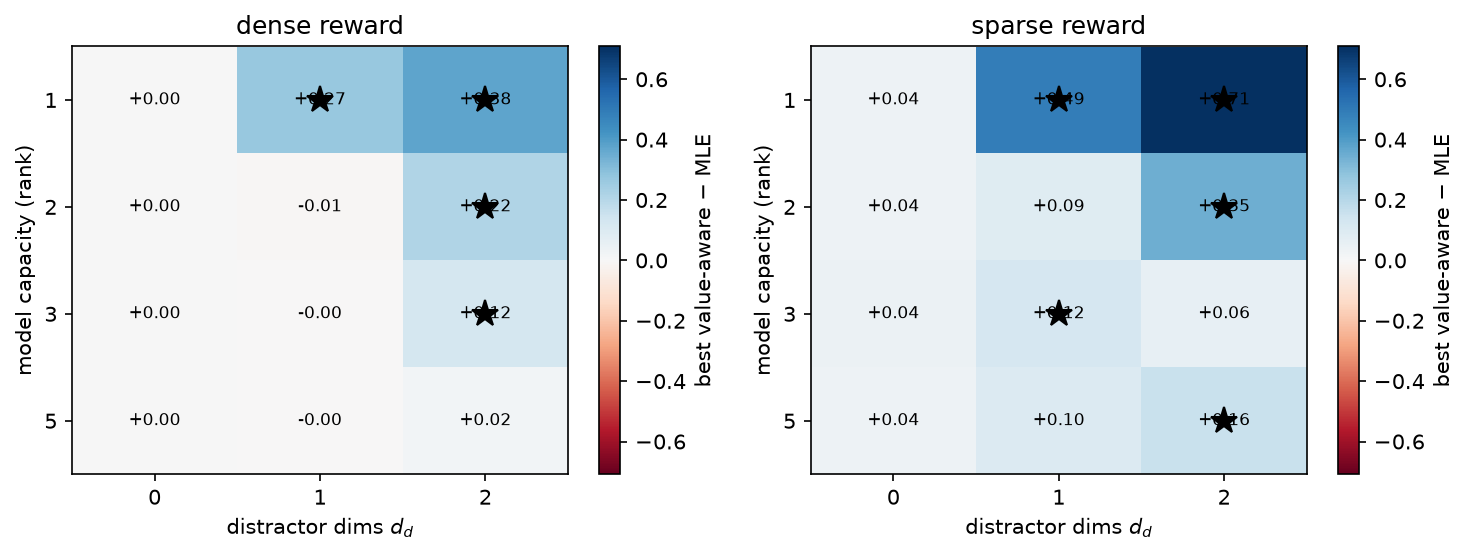
\includegraphics[width=\textwidth]{../../runs/exp5_phase/phase_diagram.png}
\caption{Mismatch phase diagram. Color is best value-aware minus MLE alignment
($\text{red}>0$: value-aware-win); stars mark value-aware-win cells. Distractors at
small capacity drive MLE below the value-aware families; larger capacity removes the
pressure. A few larger-capacity cells are seed-sensitive.}
\label{fig:phase}
\end{figure}

The structure is consistent: distractors push MLE down at small capacity and
value-aware weighting wins; raising capacity removes the pressure.

\section{Experiment 1b: Crossover and the Scope of Theorem~\ref{thm:pred}}

\begin{itemize}
\item \textbf{Uncapacitated} (\texttt{runs/exp1b}, 48 regimes): estimated-weight Bellman
  risk $\ge$ MLE in $100\%$ of regimes (VaGraM and VAML-1); oracle $\ge$ MLE in
  $94\%$/$100\%$. This validates Theorem~\ref{thm:pred} for the uncapacitated estimator.
\item \textbf{Capacity-limited} (\texttt{runs/exp1b\_capacity}, 12 regimes):
  estimated-weight risk $\ge$ MLE in only $50\%$ (VaGraM) / $33\%$ (VAML-1) of regimes.
  Reweighting a finite-capacity model changes its effective representation and can
  \emph{reduce} prediction risk, so the dominance result does not transfer
  (Remark~\ref{rem:scope}).
\end{itemize}

\begin{table}[htbp]
\centering
\caption{Theorem~\ref{thm:pred} dominance ($R_b(\hat w) \ge R_b(\text{MLE})$) by model class. The result holds for the uncapacitated estimator (Exp~1b) but not under a finite-capacity fit.}
\label{tab:scope}
\begin{tabular}{llcc}
\toprule
Model & family & regimes & $\text{est} \ge \text{MLE}$ \\
\midrule
uncapacitated & vagram & 48 & 100\% \\
uncapacitated & vaml1 & 48 & 100\% \\
capacity-limited & vagram & 12 & 50\% \\
capacity-limited & vaml1 & 12 & 33\% \\
\bottomrule
\end{tabular}
\end{table}


\section{Experiment 1.1 (deep): Policy-Gradient Alignment}
\label{sec:exp11-deep}

MuJoCo dynamics are not differentiable through the standard bindings, so the true policy
gradient is obtained by chaining per-step transition Jacobians of the \emph{real} engine:
the base task is switched to the Euler integrator and each integrator step is
differentiated with \texttt{mujoco.mjd\_transitionFD} inside a PyTorch
\texttt{autograd.Function} (\texttt{deep/mujoco\_diff.py}). A $d_d$-dimensional analytic,
reward-irrelevant distractor block is appended to the physics state. Here
$g_{\text{true}}$ is the exact rollout gradient of a fixed policy through the real
dynamics and $g_{\text{model}}$ substitutes the fitted ensemble. Datasets are
random-policy rollouts and medium-replay SAC (\texttt{runs/exp1\_deep\_alignment}, 720
rows). A normalization bug in the ensemble trainer (raw inputs at fit time, standardized
inputs at inference) had left the model underfit; after the fix the $d_d = 0$ reference
gradient is recovered.

\begin{table}[htbp]
\centering
\caption{Exp~1.1 deep policy-gradient alignment $\cos(g_{\text{true}}, g_{\text{model}})$ on the MuJoCo Distractor-Gym (differentiated via \texttt{mjd\_transitionFD}; mean over seeds and $\sigma_{\text{dist}}$); random and medium-replay SAC datasets.}
\label{tab:h11}
\begin{tabular}{llcccc}
\toprule
Dataset & $d_d$ & mle & vagram & td-error & calibrated \\
\midrule
medium & 0 & +0.061 & -0.225 & +0.427 & -0.207 \\
medium & 10 & +0.942 & +0.937 & +0.945 & +0.489 \\
medium & 50 & -0.752 & -0.760 & -0.140 & -0.445 \\
random & 0 & +0.356 & +0.796 & +0.487 & +0.196 \\
random & 10 & +0.941 & +0.934 & +0.942 & +0.941 \\
random & 50 & +0.915 & +0.903 & +0.925 & +0.810 \\
\bottomrule
\end{tabular}
\end{table}


At $d_d = 0$ alignment is high for MLE (medium $+0.92 \pm 0.10$, random $+0.74 \pm 0.37$),
confirming the diagnostic. It degrades with $d_d$ (medium $+0.79$, random $+0.55$ at
$d_d = 50$). Mean cosines are otherwise mixed, and the paired within-seed gains are
within seed noise: only calibrated on random high $d_d$ ($+0.14$/$+0.15$) and VAML-1 at
random $d_d = 10$ ($+0.17$) are positive, while every family is non-positive on medium at
$d_d = 50$ and VaGraM is $\approx 0$ everywhere. The H1.1 \emph{policy-return} claim
($\ge 40\%$ MLE degradation) is deferred to the full model-based training loop
(WP2/WP3); this section reports the gradient diagnostic.

\section{Experiment 1.2: Per-Sample VJP Profiling}
\label{sec:exp12-profiling}

We profile the per-sample value gradient $\lVert \nabla_s V(s')\rVert$ over batch sizes
$\{64, 128, 256, 512, 1024, 2048\}$ and four schemes: exact online
\texttt{torch.func.vmap(grad)}, stale-weight caching (refresh every $K \in \{5, 10, 50\}$),
central finite differences, and the forward MLE baseline
(\texttt{runs/exp1\_profiling}). On the local RTX~5060~Ti the exact VJP is
\emph{dispatch-bound} ($\sim 1$\,ms per call, roughly flat in batch), giving a
$5$--$10\times$ overhead over the forward pass and \textbf{failing H1.3} ($\le 2.2\times$
at batch $\ge 512$). Stale caching recovers it: $K = 10$ stays at $\sim 0.7$--$0.9\times$
and $K = 50$ at $\sim 0.1$--$0.2\times$; finite differences cost $140$--$220\times$ and
are not viable. This matches the plan's fallback (stale caching or a TD-error surrogate);
the plan's A100/4090 target is not available, so the overhead ratio is the reportable
quantity (Table~\ref{tab:h13}).

\begin{table}[htbp]
\centering
\caption{Exp~1.2 VJP overhead relative to the forward MLE baseline on the local RTX 5060 Ti. H1.3 (exact VJP $\le 2.2\times$ at batch $\ge 512$): FAIL (max $10.0\times$); stale caching ($K=10$) stays below the threshold.}
\label{tab:h13}
\begin{tabular}{lrrrrrr}
\toprule
Scheme & 64 & 128 & 256 & 512 & 1024 & 2048 \\
\midrule
mle-forward & 1.00 & 1.00 & 1.00 & 1.00 & 1.00 & 1.00 \\
vjp-exact & 8.31 & 8.72 & 6.49 & 8.32 & 7.14 & 10.03 \\
stale-K5 & 1.63 & 1.54 & 1.35 & 1.38 & 1.51 & 1.66 \\
stale-K10 & 0.87 & 0.68 & 0.74 & 0.71 & 0.68 & 0.86 \\
stale-K50 & 0.15 & 0.23 & 0.12 & 0.13 & 0.16 & 0.19 \\
finite-diff & 198.62 & 221.08 & 141.69 & 207.60 & 175.14 & 195.12 \\
\bottomrule
\end{tabular}
\end{table}


\section{Experiment 4: Continuous Neural Transfer (superseded)}

\textbf{Superseded by Exp~1.1 (Sec.~\ref{sec:exp11-deep}).} The earlier continuous
neural transfer used reward gradients as a value proxy and a projection loss computed in
mismatched raw vs.\ standardized coordinates. \texttt{torch} is now installed, and the
MuJoCo Exp~1.1 provides the corrected deep diagnostic; the original Exp~4 numbers
remain withdrawn.

\section{Discussion}

\textbf{When MLE fails to guide the policy.} Under goal-concentrated coverage with an
uncapacitated model, and under capacity-limited fitting with unpredictable distractors,
the model's policy gradient misaligns with the true one. Value-aware weighting that
respects the value cliff (VAML-1, Lambert) restores alignment; gradient-only VaGraM is
mis-specified when $\cos\phi$ is small or the curvature residual is large.

\textbf{Why value-aware fails.} On the uncapacitated Bellman/prediction risk it
\emph{cannot} help --- it only adds weight-noise variance --- which reproduces VaGraM's
``inferior in practice'' observation. On the decision risk it helps only when the
value-relevance signal beats the weight-noise penalty, which fails when weights are
degenerate. Under a capacity limit the two risks separate: weighting can help prediction
(by reallocating capacity), but the decision-level benefit still depends on the
weight-estimator noise.

\textbf{Practical rule of thumb.} Measure $\mathrm{SNR}_w$ and the gradient alignment
during training. If $\mathrm{SNR}_w$ is low or the alignment delta is non-positive,
value-aware weighting is not helping; the model is in the MLE-optimal regime.

\section{Limitations and Future Work}

\begin{itemize}
\item The $\mathrm{SNR}_w$ crossover statistic is a positive-but-noisy predictor, and
  the derived $\mathrm{SNR}_{\mathrm{dec}}$ is not calibrated (predicts value-aware-win
  in $100\%$ of regimes; AUC no better than $\mathrm{SNR}_w$). A closed-form threshold
  $\tau$ remains open work.
\item The phase diagram (Fig.~\ref{fig:phase}) has some seed-sensitive cells at larger
  capacity; more seeds and a finer capacity sweep are needed to tighten it.
\item The tabular results are stylized. The continuous transfer (Exp~4) is superseded by
  the MuJoCo Exp~1.1; the original raw vs.\ standardized coordinate bug is removed by
  construction, and the earlier Exp~4 numbers stay withdrawn.
\item The Exp~1.1 deep diagnostic measures policy-gradient \emph{alignment}, not policy
  \emph{return}; the H1.1 return claim needs the full model-based training loop.
\item The Exp~1.2 profiling runs on a local RTX~5060~Ti, not the plan's A100/4090, so it
  reports the VJP overhead ratio rather than absolute throughput; exact VJP fails H1.3 on
  this setup while stale-weight caching meets it.
\item The distractor bandwidth/capacity interaction is sensitive; more seeds and a
  systematic capacity sweep are needed to tighten the phase diagram.
\item Phase~2: the diagnostics must be ported to MBPO, DreamerV3, TD-MPC2, and VaGraM
  (benchmark provisioning is an open item; \texttt{mbrl-lib} pins old \texttt{gym}).
\end{itemize}

\bibliographystyle{plain}
\bibliography{../shared/references}

\end{document}
